\documentclass[journal]{IEEEtran}

% Packages
\usepackage{cite}
\usepackage{amsmath,amssymb,amsfonts}
\usepackage{algorithmic}
\usepackage{graphicx}
\usepackage{textcomp}
\usepackage{xcolor}
\usepackage{float}
\usepackage{pgfplots}
\usetikzlibrary{pgfplots.polar}


% Title
\title{Exploring the Impact of Interactive Advertisements on User Experience: An Evaluation of Different Types of  Ads}

\author{Aayush Pokharel,
Sushant Regmi,
Subash Khatri,
    Sabin Badal,
    and Ranjit Sapkota}

\begin{document}

\maketitle

\begin{abstract}
    This research project aims to investigate the impact of interactive
    advertisements on user experience by evaluating various types of ads.
    Traditional advertising methods often irritate users and fail to
    effectively promote brands, products, or services. In response to
    these challenges, this study focuses on interactive ads, which provide
    engaging and interactive experiences for users. By evaluating different
    types of interactive ads, we seek to understand their potential to
    enhance user experience and overcome the limitations of conventional
    advertising methods. The research team will employ a mixed-methods
    approach, combining qualitative and quantitative research techniques.
    The evaluation will involve user surveys, interviews, and usability
    testing to gather data on user preferences, engagement levels, brand
    recall, and perception. Through statistical analysis and thematic coding,
    the findings will provide insights into the effectiveness and user
    experience of different interactive ad formats. The expected outcomes of
    this research include a comprehensive understanding of how interactive ads
    influence user experience, user engagement, brand recall, and brand perception.
    The research findings will contribute to the development of more effective
    and user-friendly advertising strategies that prioritize user experience
    and engagement. Furthermore, the research aims to provide actionable insights
    to advertisers and marketers seeking to improve the effectiveness of their
    advertising campaigns. By exploring the impact of interactive advertisements,
    this research project contributes to the advancement of advertising practices
    and aligns with the evolving needs and preferences of users in the digital age.
    The results of this study will not only benefit marketers and advertisers but
    also enhance the overall user experience in the advertising ecosystem.
\end{abstract}

\begin{IEEEkeywords}
    HCI, User Experience, User Interface, Static Ads, Interactive Ads,
\end{IEEEkeywords}

\section{Introduction}
\subsection{Background}
\IEEEPARstart{I}{n} today's digital landscape, advertisements play a pivotal role in promoting brands,
products, and services. However, the effectiveness of traditional advertising methods
has been increasingly questioned as users grow more resistant to intrusive and
irrelevant ads\cite{shavitt1998public}. Traditional approaches, such as
banner ads or pop-ups, often fail to captivate users' attention, leading to reduced
engagement, limited brand recall, and suboptimal outcomes for advertisers. As a result,
there is a growing need to explore alternative advertising strategies that prioritize
user experience and engagement.

\subsection{Motivation}
This research project focuses on exploring the impact of interactive advertisements on user experience.
Interactive ads, characterized by their ability to provide engaging and interactive experiences,
have emerged as a potential solution to the limitations of traditional advertising methods \cite{roy2020role}.
By incorporating gamification, personalized content, and interactivity, these ads aim to establish
meaningful connections with users and deliver persuasive messages. Understanding the effectiveness
of interactive ads in promoting brands, products, or services is crucial for advertisers and
marketers seeking more effective and user-friendly advertising strategies.

\subsection{Literature Review}
Interactive advertising has emerged as a highly effective approach, captivating viewers and driving
brand awareness with greater efficacy than static advertising \cite{petty1986communication}. The Elaboration
Likelihood Model (ELM) provides insights into the psychological processes underlying the effectiveness
of interactive ads.It posits that interactive ads, by offering opportunities for interaction and
engagement, stimulate central processing, leading to profound message elaboration and favorable brand attitudes.

The Theory of Planned Behavior (TPB) further highlights the factors influencing consumer behavior
and the effectiveness of interactive ads\cite{ajzen1991theory}. Interactive ads impact elements of the TPB, including
intention, perceived behavioral control, and attitude. These ads enhance intention by making behaviors more
captivating, improve perceived behavioral control by increasing ease and accessibility, and shape attitudes
by making behaviors more desirable and eliciting positive evaluations.

The Social Cognitive Theory (SCT) emphasizes observational learning and suggests that interactive ads can
serve as models for desired behavior\cite{bandura1986social}. By showcasing positive outcomes associated with the
behavior, interactive ads inspire consumers to seek similar experiences. The SCT reinforces the notion that
interactive ads hold greater sway in influencing consumer behavior compared to non-interactive ads.

The Interactivity Theory delves deeper into the role of interactivity in advertising\cite{liu2002interactivity}.
It posits that interactivity engenders a sense of control, involvement, and engagement among viewers,
transcending the passive nature of static ads. Interactive ads captivate attention and foster deeper
engagement by actively involving viewers and allowing them to shape their own experiences.

The Social Presence Theory highlights the impact of social interaction in advertising\cite{short1976social}.
Interactive ads incorporating features facilitating social interaction amplify the sense of social presence, fostering greater
engagement and involvement among viewers.

Supporting these theoretical perspectives, empirical evidence from Natalia Viktorovna Antonova's study (2015) titled
"The Psychological Effectiveness of Interactive Advertising"\cite{antonova2015psychological} confirms the empowering effect of interactivity
on individuals, enabling them to identify with advertising characters and actively participate within
the advertising environment. Active involvement in interactive ads increases individuals'
willingness to act in the real world, enhancing the potential impact of interactive
advertising on consumer behavior and brand perception.

In conclusion, the Elaboration Likelihood Model, Theory of Planned Behavior, Social Cognitive Theory,
Interactivity Theory, and Social Presence Theory collectively demonstrate the effectiveness of interactive
advertising in fostering engagement and brand awareness. These theoretical frameworks, supported by empirical
evidence, highlight the psychological impact of interactivity in shaping consumer behavior and conveying
brand messages effectively. Interactive ads, by fostering central processing, interactivity, social
interaction, intention, perceived behavioral control, attitude, and observational learning,
drive greater brand engagement. As interactive advertising continues to evolve, its importance
as a powerful marketing tool becomes increasingly evident.

\subsection{Problem Statement}
The problem at hand encompasses two main aspects. Firstly, there is a need to assess the
effectiveness of interactive advertisements in engaging users and facilitating brand
recall, comprehension of product claims, and risk disclosures. Secondly, it is
crucial to address the potential irritations and negative experiences that
users may encounter when interacting with such ads. By understanding the challenges
and opportunities associated with interactive advertising, we can develop strategies
to optimize these ads and improve user experience, leading to desired advertising
outcomes.

To tackle these concerns, this research project aims to investigate the impact of
interactive advertisements on user experience by evaluating different types of ads.
By examining user engagement, recall, comprehension, and potential irritations, the
study seeks to provide valuable insights for advertisers, marketers, and designers
to enhance the effectiveness of interactive advertising campaigns.

\subsection{Research Question}
This research project aims to investigate the impact of interactive advertisements
on user experience and advertising effectiveness. To achieve this, the study will
address the following research questions:

\begin{itemize}
    \item How do user attitudes and perceptions towards interactive advertisements influence their engagement and recall of advertised brands?
    \item What are the key factors that contribute to user comprehension of product claims and risk disclosures in interactive advertisements?
    \item How do different types of interactive ad formats (e.g., gamification, personalized content) affect user experience and engagement?
    \item What are the potential irritations and negative experiences that users may encounter when interacting with interactive advertisements, and how can they be mitigated?
\end{itemize}

\subsection{Research Objective}
The primary objective of this study is to comprehensively evaluate the impact of
interactive advertisements on user experience. To achieve this, we will assess various types
of interactive ads to understand their effectiveness in engaging users, enhancing brand recall,
and improving overall brand perception \cite{giombi2022impact}. By employing a mixed-methods approach,
combining qualitative and quantitative research techniques, we aim to gather robust data
to achieve the following objectives:
\begin{itemize}
    \item Investigate the relationship between user attitudes and perceptions towards interactive advertisements and their engagement and recall of advertised brands.
    \item Identify the key factors that contribute to user comprehension of product claims and risk disclosures in interactive advertisements.
    \item Examine how different types of interactive ad formats (e.g., gamification, personalized content) affect user experience and engagement.
    \item Explore the potential irritations and negative experiences that users may encounter when interacting with interactive advertisements and develop strategies to mitigate them.
\end{itemize}
By pursuing these research objectives, we aim to generate valuable insights and practical knowledge that can contribute to the advancement of
interactive advertising practices. Ultimately, the objective is to create more engaging, user-friendly, and
persuasive interactive advertisements that align with user preferences and needs, resulting in improved user experiences and advertising outcomes.


\subsection{Significance}
The outcomes of this research hold significant potential for advertisers and marketers
seeking more effective and user-friendly advertising strategies. By gaining insights into
how interactive ads influence user experience, engagement, and brand perception, advertisers
can tailor their campaigns to better resonate with their target audience \cite{sundar2008main}.
Moreover, understanding the impact of interactive ads on user experience can pave the way
for the development of innovative and engaging advertising approaches that prioritize user preferences and needs.

\subsection{Research Approach}
To accomplish our research goals, we will employ a range of research methods, including user
surveys, interviews, and usability testing. The collected data will be subjected to rigorous
statistical analysis and thematic coding, allowing us to draw meaningful conclusions and insights.
It is essential to emphasize that the research findings are intended to provide actionable
insights and recommendations to advertisers and marketers looking to enhance the
effectiveness of their advertising campaigns \cite{liang2008user}.

\subsection{Outline}
In summary, this research project aims to contribute to the advancement of advertising
practices by exploring the impact of interactive advertisements on user experience. By
evaluating various types of ads, we seek to identify effective strategies that can address
the limitations of traditional advertising methods and create engaging experiences for users.
The results of this study have the potential to reshape advertising practices, improve user
experience, and foster a more harmonious relationship between advertisers and their target audience.


\section{Methodology}
This section presents the methodological framework employed in this research study, which
encompasses survey research, experimental design, content analysis, and user interviews.
These methodological approaches have been carefully selected to comprehensively investigate
the impact of interactive advertisements on user experience, engagement, comprehension,
and potential irritations. By combining both quantitative and qualitative techniques,
this study aims to provide a thorough and rigorous analysis of the research topic.

\subsection{User interviews and Focus Groups}
To validate the clarity of our research questions, a think aloud session was conducted
with a focus group comprising five individuals who were familiar with the field of HCI.
The purpose of this session was to engage participants in a discussion about our research
ideas and solicit their feedback on the research questions.

During the session, participants were presented with the research questions and prompted
to share their perspectives. They were asked open-ended questions to assess the clarity
and comprehensibility of the research questions. Specifically, participants were asked:

\begin{itemize}
    \item "Did you find the research question clear and easy to understand?"
    \item "Was there anything about the research question that was confusing or unclear to you?"
    \item "Do you think the research question accurately captures the main objective of this study?"
\end{itemize}

The think aloud session provided an opportunity for participants to openly express their
thoughts, opinions, and any concerns they had regarding the clarity and accuracy of the
research questions. Their responses were carefully documented and analyzed to gain
insights into their understanding and perceptions.

The inclusion of a focus group in the think aloud session allowed for a diverse range of
perspectives to be considered. By engaging multiple participants, we aimed to ensure
a comprehensive evaluation of the clarity of the research questions. The insights
gained from the think aloud session were used to refine and clarify the research
questions as necessary, ensuring their effectiveness in addressing the objectives of
the study.

The think aloud session with the focus group served as a valuable step in the methodology,
providing a rigorous approach to validate and enhance the clarity of the research
questions. The session's findings were considered alongside other validation techniques
to ensure the robustness and accuracy of our research objectives.

\subsection{Content Analysis}
To ensure the relevance and cultural appropriateness of the advertisements for our target
audience in Nepal, a systematic sample selection process was conducted. We specifically
chose advertisements that were targeted towards the Nepalese audience or originated from
the Nepalese market. The selection criteria included prominent platforms such as Daraz NP
and Ncell, which are widely recognized in Nepal. The chosen advertisements predominantly
adopted a static format, allowing for a detailed analysis of their visual and textual content.

By aligning our sample with the customs, habits, and culture of the Nepalese population,
we aimed to obtain more meaningful insights and accurate findings that can be applied in
the context of Nepal. The selected advertisements were carefully evaluated to ensure they
catered to the preferences and cultural nuances of the Nepalese audience. By incorporating
locally produced ads and those specifically designed for the Nepalese market, we captured
the unique characteristics and sociocultural aspects that influence consumer behavior in
Nepal.

\begin{figure}[H]
    \centering
    \includegraphics[width=8cm]{daraz-sale.png}
    \caption{A DarazNP ad promoting 1111 sale on website.}
\end{figure}

\begin{figure}[H]
    \centering
    \includegraphics[width=8cm]{Ncell.png}
    \caption{A Ncell ad for it's data service.}
\end{figure}

The content analysis process involved a systematic examination of the selected
advertisements. Drawing upon established research objectives and relevant literature, a
comprehensive set of coding categories was developed.
\clearpage
These categories encompassed various aspects like:
\begin{itemize}
    \item including visual elements
    \item textual messages
    \item product features
    \item cultural references
    \item emotional appeals
\end{itemize}
Individual researchers independently coded the advertisements, ensuring consistency and
minimizing potential biases. Any discrepancies or uncertainties were resolved through
rigorous discussions and consensus among the research team.

By employing content analysis, we gained valuable insights into the selected advertisements,
paving the way for subsequent stages of our research. These insights serve as a foundation
for assessing user engagement and further data interpretation, enabling us to explore the
influence of these advertisements on user behavior and perceptions.

\subsection{Experimental Design}
Interactive versions of the selected advertisements were developed to facilitate further
investigation and analysis. These prototypes aimed to enhance user engagement by incorporating
interactive elements of mapping and gamification aspects. To ensure the feasibility and practicality of
the prototypes, a paper-based prototyping approach was initially utilized.

Gamification techniques were strategically employed to enhance user interaction, motivation,
and enjoyment. The prototypes were designed to offer users a rewarding and immersive experience
through interactive features such as personalized content.

To expedite the iterative design process and gather feedback, paper prototypes were created as a
preliminary representation of the interactive ads. Paper prototypes allowed for quick modifications,
adaptations, and refinements based on the discussion of group members. This approach facilitated the
exploration of various design possibilities and the identification of potential issues or areas for
improvement before transitioning to digital prototypes.

\begin{figure}[H]
    \centering
    \includegraphics[height=7cm]{dp1.jpg}
    \caption{Paper prototype of daraz NP ads showing download button}
\end{figure}

\begin{figure}[H]
    \centering
    \includegraphics[height=5cm]{dp4.jpg}
    \caption{second iteration of prototype ads showing download button}
\end{figure}

\begin{figure}[H]
    \centering
    \includegraphics[height=7cm]{dp2.jpg}
    \caption{Paper prototype of daraz NP ads showing 360\textdegree{} product demo.}
\end{figure}

\begin{figure}[H]
    \centering
    \includegraphics[height=7cm]{dp3.jpg}
    \caption{Paper prototype of daraz NP ads showing gamification aspects}
\end{figure}

\begin{figure}[H]
    \centering
    \includegraphics[height=7cm]{dp5.png}
    \caption{prototype ad that combined download and 360\textdegree{} product demo.}
\end{figure}

\begin{figure}[H]
    \centering
    \includegraphics[width=8cm]{ncell1.jpg}
    \caption{prototype ad that used mapping to deliver personalized content}
\end{figure}

\begin{figure}[H]
    \centering
    \includegraphics[width=8cm]{ncell2.jpg}
    \caption{second iteration of prototype Ncell ad that used mapping}
\end{figure}

\begin{figure}[H]
    \centering
    \includegraphics[height=6cm]{chess1.jpg}
    \caption{paper prototype of a chess game ad that can be played.}
\end{figure}

\begin{figure}[H]
    \centering
    \includegraphics[height=6cm]{chess2.jpg}
    \caption{paper prototype of a chess game ad prompting interaction}
\end{figure}

\begin{figure}[H]
    \centering
    \includegraphics[height=6cm]{chess3.jpg}
    \caption{Second iteration of prototype of a chess game}
\end{figure}

\begin{figure}[H]
    \centering
    \includegraphics[height=6cm]{chess4.jpg}
    \caption{prototype showing the interactive hint in chess game}
\end{figure}

The subsequent redesign iterations based on paper prototyping findings paved the way for the final
digital versions of the interactive ads to be used in the upcoming survey.

\subsection{Survey Research}

In order to facilitate our study, the test group was divided into two cohorts:
\begin{itemize}
    \item HCI conscious cohort
    \item HCI unconscious cohort
\end{itemize}
The HCI conscious cohort consisted of individuals who were familiar with the
topic of Human-Computer Interaction (HCI) and possessed a basic understanding
of Shneiderman's Eight Golden Rules. On the other hand, the HCI unconscious
cohort comprised the remaining members of the test group.

To assess user engagement levels during the interactive experience, we employed
the User Engagement Scale (UES) questionnaire. This questionnaire is specifically
designed to measure users' engagement levels during interactive encounters. \cite{obrien2008user}
It utilizes the Likert Scale \cite{likert1932technique}, a commonly used rating scale, as well as frequency scale for participants
to provide their responses.

The utilization of these cohorts and the UES questionnaire with Likert Scale
responses enabled us to gather valuable insights into the engagement levels
of both HCI conscious and HCI unconscious participants. These findings contributed
to the comprehensive analysis of user engagement within the context of our study.

\section{Experimental Results}
This section presents the findings of our research, which employed a multifaceted
approach encompassing user interviews, focus groups, content analysis, experimental
design, and survey research. Utmost attention was devoted to ensuring the accuracy,
uniqueness, completeness, timeliness, and understandability of the collected data.

\subsection{User interviews and Focus Groups}
In this study, semi-structured interviews was conducted with a cohort of 5 participants to gain valuable
insights into their experiences and perceptions related to the research topic. Additionally,
focus groups were employed to facilitate dynamic group discussions and capture a diverse
range of perspectives.

Through interviews and focus groups, a number of themes emerged concerning the transition
of an advertisement from being static to interactive, particularly in terms of the necessity
of clicking. Specifically, the question of whether clicking on an ad constitutes a form of
interaction was explored.

The unanimous consensus among participants was that clicking on an ad was indeed considered
a form of interaction. However, participants emphasized that simply presenting an ad in an
infographic format and requiring a click did not inherently qualify the ad as interactive.

These findings, obtained through qualitative analysis, provide significant insights into
the  perspectives of the participants.

% \subsection{Content Analysis}

\subsection{Experimental Design}
After the completion of the paper prototype development and finalization of the design,
the subsequent phase involved the implementation of viable interactive ads.

The following designs were selected as part of this process.

\begin{figure}[H]
    \centering
    \includegraphics[height=7cm]{Daraz360.png}
    \caption{DarazNP 360\textdegree{} Product Demo Ad}
\end{figure}
In this particular instance, the advertisement leverage the cognitive bias known as the
Serial Position Effect to influence the end user's behavior. By strategically placing the
download button on the lower right of the screen, the ads take advantage of the tendency
for individuals to have a stronger memory and preference for items positioned at the end
of a series. This positioning aims to increase the likelihood of users clicking the
download button to acquire the application.

Additionally, the advertisements employ the principles of the Law of Proximity, which is
based on gestalt psychology. By utilizing the spatial arrangement of the display items,
the ads create a visual grouping effect to indicate that a particular element is an
interactible 3D model. The proximity between the interactive element and other related
visual elements helps users perceive their relationship and interpret the interactive
nature of the model.

By incorporating these psychological principles into the design of the ads, they aim to
enhance user engagement and guide user behavior towards the desired action, such as
downloading the app. The application of these cognitive and perceptual principles
demonstrates a strategic approach to design that leverages psychological mechanisms to
influence user interactions and achieve specific objectives.

\begin{figure}[H]
    \centering
    \includegraphics[height=7cm]{DarazScratch1.png}
    \caption{DarazNP Scratch Ad}
\end{figure}

\begin{figure}[H]
    \centering
    \includegraphics[height=7cm]{DarazScratch2.png}
    \caption{DarazNP Scratch Ad showing the personalized discount}
\end{figure}

In this specific scenario, the advertisement capitalizes on the cognitive bias
referred to as the Von Restorff Effect to shape the end user's behavior and capture
their attention. The advertisement achieves this by employing a distinct visual element,
such as text in a different color, that prompts the user to engage in an action—specifically,
scratching—to reveal a hidden discount. Subsequently, the revealed content displays the
discounted percentage.

By leveraging the Von Restorff Effect, which emphasizes the memorability of distinctive
and novel stimuli, the advertisement aims to stand out and create a memorable impression
on the user. The use of color contrast and the interactive scratching action work in conjunction
to draw the user's attention and generate curiosity. This approach is strategically employed to
enhance user engagement and increase the likelihood of the desired behavior—revealing and
ultimately availing the discount.

\begin{figure}[H]
    \centering
    \includegraphics[height=7cm]{HCI-CHESS1.jpg}
    \caption{Chess game ad prompting user interaction to play}
\end{figure}

\begin{figure}[H]
    \centering
    \includegraphics[height=7cm]{HCI-CHESS2.jpg}
    \caption{Chess game ad prompting user to check for hint}
\end{figure}

\begin{figure}[H]
    \centering
    \includegraphics[height=7cm]{HCI-CHESS3.jpg}
    \caption{Chess game ad prompting user to download the app}
\end{figure}

In this particular context, the advertisement strategically utilizes two cognitive biases,
namely the Von Restorff Effect and the Serial Position Effect, to influence user behavior
and attract their attention. The application of these biases involves placing a hint
at the last position within the advertisement while employing distinct coloring to make
it stand out from its surroundings. This deliberate arrangement aims to invoke attention
and enhance the memorability of the hint.

Furthermore, the advertisement incorporates the concept known as Parkinson's Law by
incorporating a time-based element. Specifically, a timer is introduced to create a sense
of urgency and prompt users to engage with a chess puzzle within a designated time frame.
By leveraging Parkinson's Law, which suggests that work expands to fill the time available,
the advertisement seeks to motivate users to actively participate and solve the puzzle within
the given time constraint.

\begin{figure}[H]
    \centering
    \includegraphics[width=8cm]{ncell_slide.png}
    \caption{Ncell ad that used mapping to provide a customized experience}
\end{figure}

In this specific scenario, the advertisement employs a heuristic approach known as Miller's
effect to enhance user experience and decision-making. This approach involves limiting the
number of options on a slider to only five, aiming to simplify the decision-making process
for the user. By reducing the number of choices, the advertisement mitigates cognitive load
and facilitates quicker decision-making.

Furthermore, the advertisement incorporates Hick's law, which suggests that increasing the
number of choices leads to longer decision-making times. To optimize user decision-making,
the advertisement carefully minimizes the available choices and emphasizes a recommended
option. By doing so, the advertisement streamlines the decision-making process and guides
users towards the most favorable choice.

\subsection{Survey Research}
Multiple surveys were conducted to assess the viability and accuracy of the problem statement.
The initial survey aimed to evaluate the problem statement and gather feedback. A total of
32 individuals participated in this survey, and the test audience was divided into two
distinct cohorts: HCI-conscious and HCI-unconscious.



\begin{figure}[ht]
    \centering
    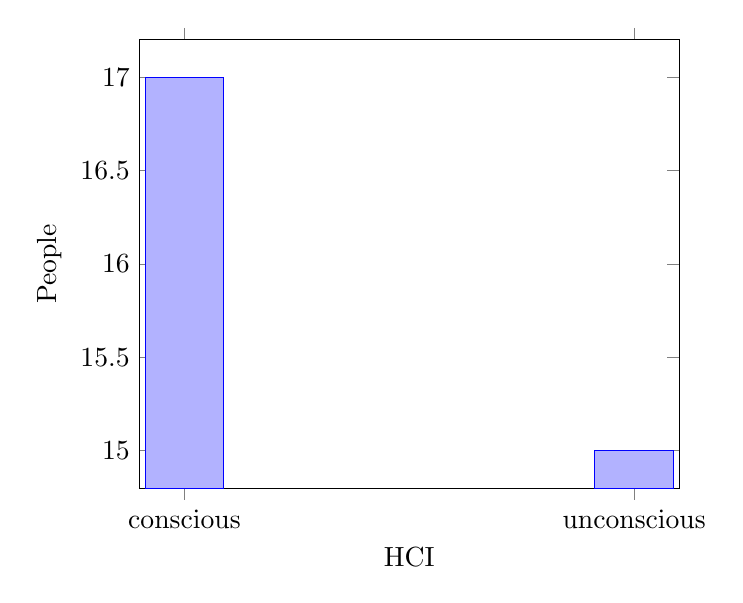
\begin{tikzpicture}
        \begin{axis}[
                ybar,
                bar width=1cm,
                xlabel={HCI},
                ylabel={People},
                xtick=data,
                xticklabels={conscious, unconscious},
                legend style={at={(0.5,-0.15)}, anchor=north, legend columns=-1},
            ]
            \addplot coordinates {(1,17) (2,15)};
        \end{axis}
    \end{tikzpicture}
    \caption{Demographic of HCI conciousness in test group}
\end{figure}

\begin{figure}[ht]
    \centering
    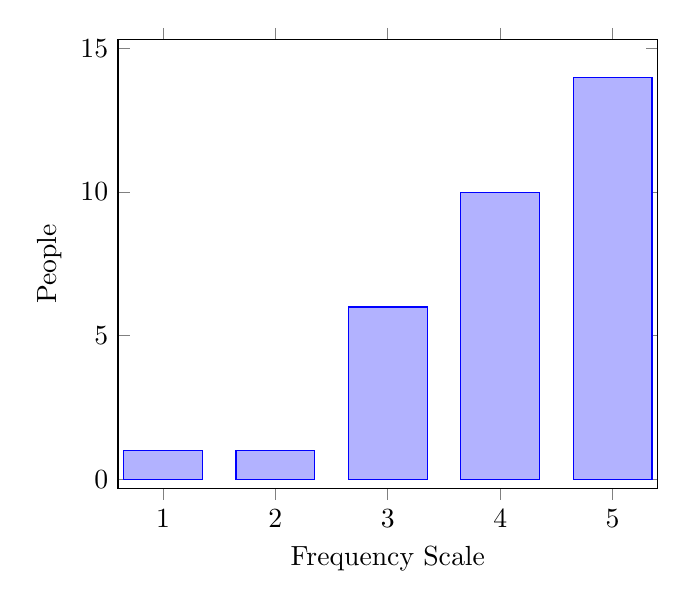
\begin{tikzpicture}
        \begin{axis}[
                ybar,
                bar width=1cm,
                xlabel={Frequency Scale},
                ylabel={People},
                xtick=data,
                xticklabels={1, 2, 3,4,5},
                legend style={at={(0.5,-0.15)}, anchor=north, legend columns=-1},
            ]
            \addplot coordinates {(1,1) (2,1) (3,6) (4,10) (5,14)};
        \end{axis}
    \end{tikzpicture}
    \caption{How often do you encounter ads?}
\end{figure}

\clearpage

\begin{figure}[ht]
    \centering
    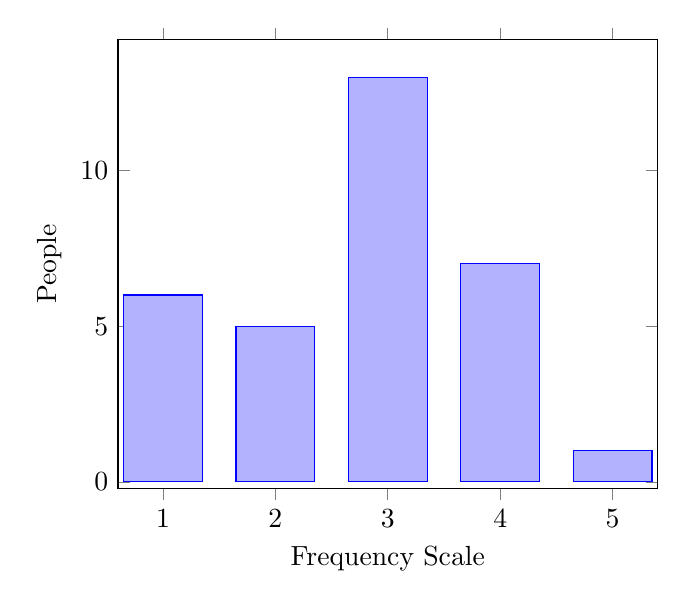
\begin{tikzpicture}
        \begin{axis}[
                ybar,
                bar width=1cm,
                xlabel={Frequency Scale},
                ylabel={People},
                xtick=data,
                xticklabels={1, 2, 3,4,5},
                legend style={at={(0.5,-0.15)}, anchor=north, legend columns=-1},
            ]
            \addplot coordinates {(1,6) (2,5) (3,13) (4,7) (5,1)};
        \end{axis}
    \end{tikzpicture}
    \caption{Do you enjoy ads?}
\end{figure}

Once the paper prototypes were completed, incorporating the newly designed interactive
ads, a comparative study was conducted to measure user engagement. This study involved
a sample survey where the ads were distributed to individuals who had previously
participated in the survey.

The aim of this comparative study was to assess the level of user engagement elicited
by the different ad designs. By leveraging the sample survey, we could gather valuable
feedback from participants who had already provided their insights on the survey
questions. This approach allowed us to gain a deeper understanding of how the new
interactive ads influenced user engagement, taking into consideration the respondents'
prior exposure to the survey content.

By employing this methodology, we could effectively analyze the user engagement metrics
and compare the results between different ad designs. The insights obtained from this
comparative study served as a crucial foundation for evaluating the effectiveness of
the new interactive ads and informing further iterations in the design process.

\begin{figure}[ht]
    \centering
    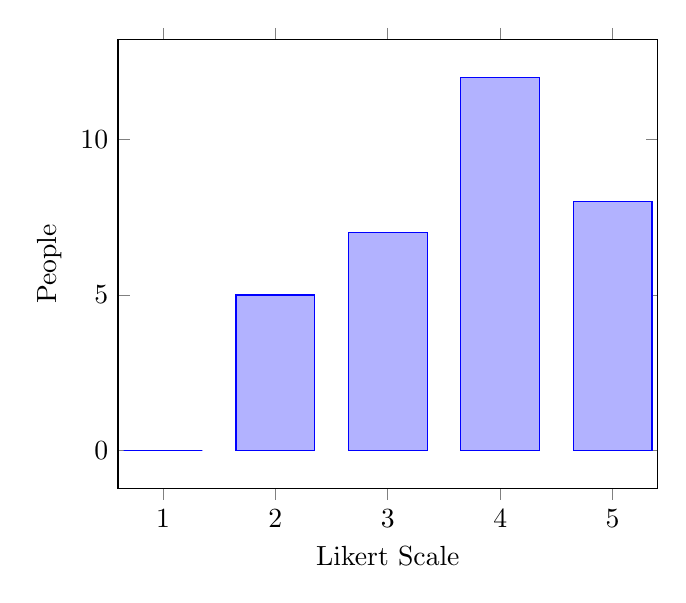
\begin{tikzpicture}
        \begin{axis}[
                ybar,
                bar width=1cm,
                xlabel={Likert Scale},
                ylabel={People},
                xtick=data,
                xticklabels={1, 2, 3,4,5},
                legend style={at={(0.5,-0.15)}, anchor=north, legend columns=-1},
            ]
            \addplot coordinates {(1,0) (2,5) (3,7) (4,12) (5,8)};
        \end{axis}
    \end{tikzpicture}
    \caption{The interaction with the ad was meaningful and personally relevant. }
\end{figure}

\begin{figure}[ht]
    \centering
    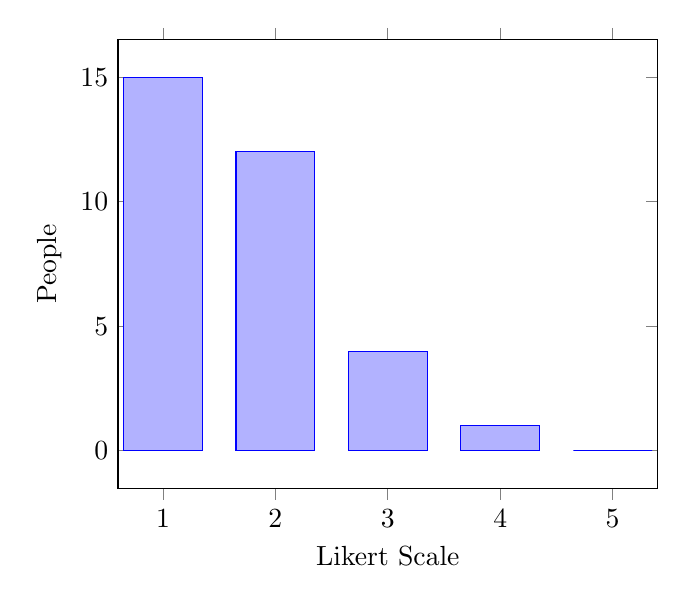
\begin{tikzpicture}
        \begin{axis}[
                ybar,
                bar width=1cm,
                xlabel={Likert Scale},
                ylabel={People},
                xtick=data,
                xticklabels={1, 2, 3,4,5},
                legend style={at={(0.5,-0.15)}, anchor=north, legend columns=-1},
            ]
            \addplot coordinates {(1,15) (2,12) (3,4) (4,1) (5,0)};
        \end{axis}
    \end{tikzpicture}
    \caption{Mental effort had to be exert to use the system. }
\end{figure}

\begin{figure}[ht]
    \centering
    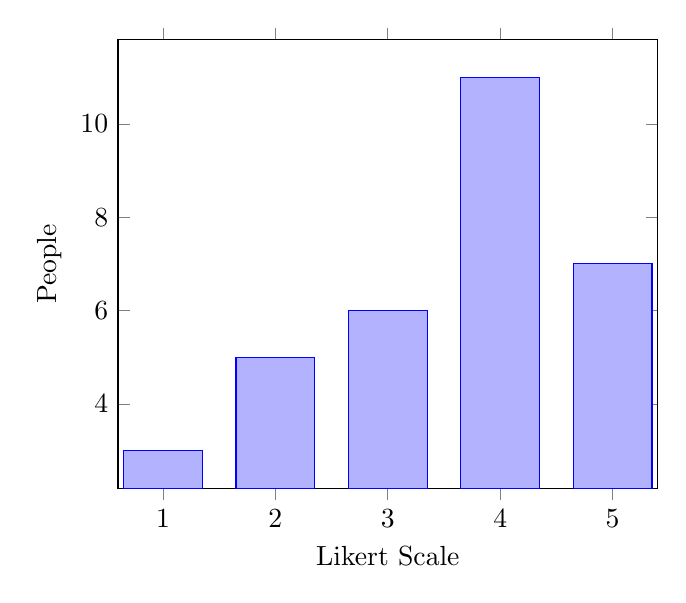
\begin{tikzpicture}
        \begin{axis}[
                ybar,
                bar width=1cm,
                xlabel={Likert Scale},
                ylabel={People},
                xtick=data,
                xticklabels={1, 2, 3,4,5},
                legend style={at={(0.5,-0.15)}, anchor=north, legend columns=-1},
            ]
            \addplot coordinates {(1,3) (2,5) (3,6) (4,11) (5,7)};
        \end{axis}
    \end{tikzpicture}
    \caption{The ads gave proper amount of control to the user. }
\end{figure}
7

\section{Discussion}
The findings from the survey data strongly indicate a lack of favorability towards
static ads among participants, highlighting their unappealing nature and lack of
engagement. However, the results also reveal a notable interest and willingness
among respondents to interact with interactive ads, provided they are visually
captivating and engaging. These findings align with our initial problem statement,
emphasizing the need to explore alternative advertising strategies that prioritize
user experience and engagement as engagement resulted in positive attitude towards ads.

The survey results also showed that proper grouping of the ads resulted a clearer discource of
information and through the use of mapping, comprehension of product claims could be easily achieved.
This also serve as validation for the significance of incorporating interactivity and engaging elements in advertisements to capture the attention
and interest of the target audience. This aligns with our objective of developing innovative solutions
and addressing the limitations associated with traditional advertising methods.

Equipped with these valuable insights, we can confidently claim that level of control is directly
tied with potential irritations and inadequate amount of it may result in a negative experience just like in the
case of static ads.

With a better understanding of users' preferences and expectations,
we can now focus on designing and implementing interactive ad campaigns that leverage personalization,
to establish meaningful connections with our target audience.


\section*{Acknowledgment}
The authors would like to acknowledge the support and contributions of various
individuals and organizations in the completion of this research paper. We
express our sincere gratitude to the Kathmandu University for providing the
opportunity to pursue the BSc. degree in Computer Science.

Special thanks are extended to Assistant Professor Dr. Sushil Shrestha for
his invaluable guidance, expertise, and continuous support throughout the
research process. His constructive feedback, insightful suggestions, and
profound knowledge in the field of Human-Computer Interaction (HCI) have
significantly influenced the quality and direction of this research.

We would also like to acknowledge the assistance and cooperation received
from the  Kathmandu University. Their support in providing access to essential
resources, including the library facilities, is greatly appreciated.

Furthermore, we would like to express our gratitude to our fellow classmates
for their valuable collaboration, discussions, and shared experiences during
the course. Their diverse perspectives have enriched our research work and
broadened our understanding of HCI.

Finally, the authors would like to thank all the participants who generously
contributed their time and insights to this research study. Their participation
has been crucial in collecting the necessary data and ensuring the validity of
our findings.

The authors acknowledge the contributions and support provided by all the
individuals and organizations mentioned above. Their involvement has been
instrumental in the successful completion of this research.

\ifCLASSOPTIONcaptionsoff
    \newpage
\fi

\bibliographystyle{IEEEtran}
\bibliography{references}

\end{document}
